The market research and the estimations of the cost per dose done with the bioreactor considered at the beginning of the project were just considering the facilities, such as water and electricity, and the working volume per batch. However, the vaccine production process comprehends also other relevant step which were not considered in the first place. The vaccine in fact needs to undergo also a  purification process which is made up of three different sections. First the proteins grown in the bioreactor need to be isolated from the rest of the solution, to do so two different methods are applied, which are the centrifugation and homogenisation. However, the isolated solution will still have carried over some debris which needs to be removed during the second step called purification. During this part first microfiltration and ultrafiltration are used to remove suspended particles, microorganism and fats and after chromatography is used to filter the desired protein from the remaining binding material and non-binding protein. Finally, there is the finishing of the product during which the vaccine takes the form decided, such as tablets or injection. The following diagram show this process and the usual number of operations needed.
\begin{figure}
    \centering
    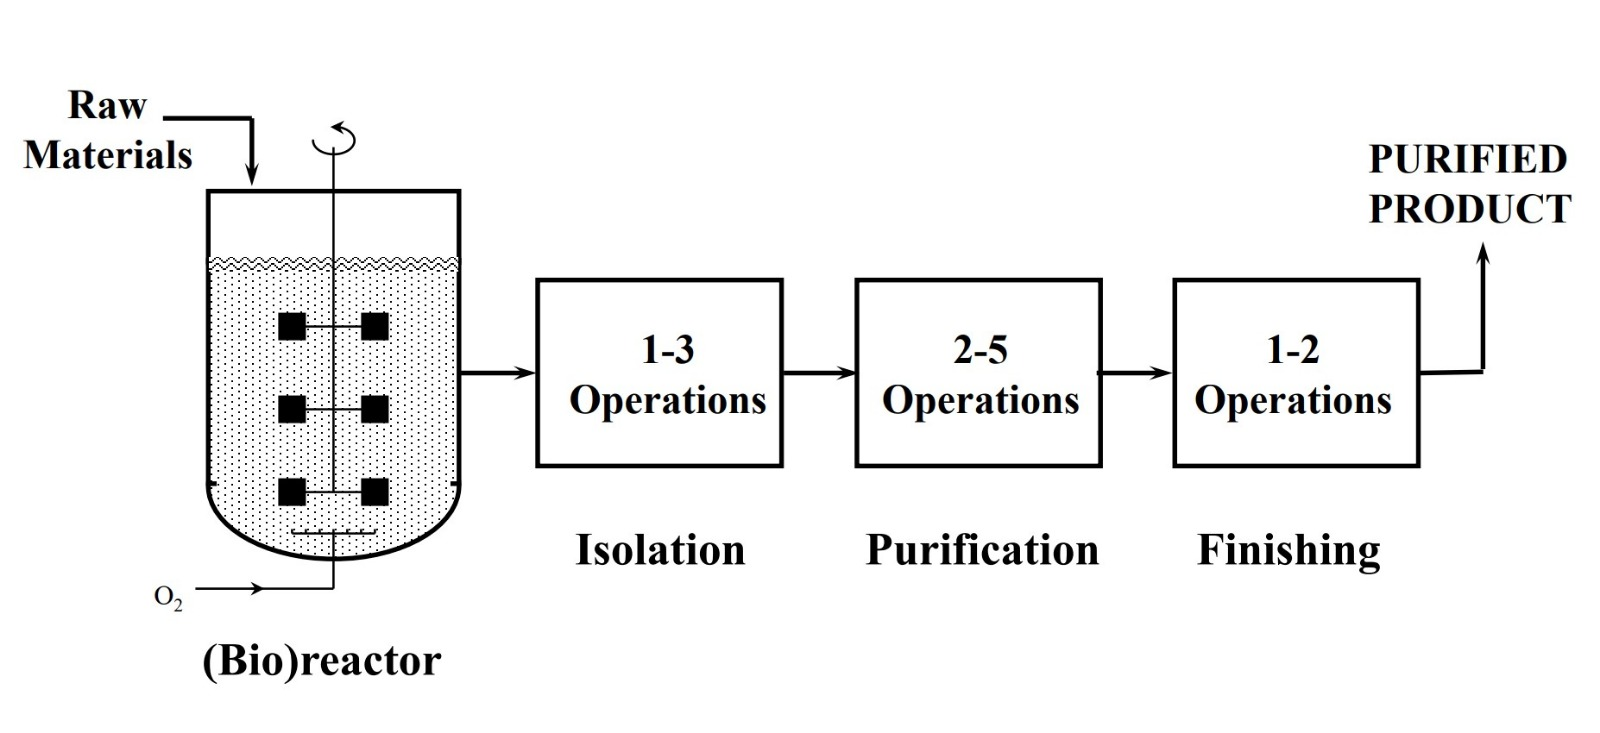
\includegraphics[width=0.5\textwidth]{design-process.jpeg}
\end{figure}

In order to calculate the final cost per dose of a vaccine dose some scale-up calculations were required. By looking at the following process flowsheet where the units have been specified for a 3000 L bioreactor and assuming that the cost and size of the equipment correlate linearly with the bioreactor capacity, a simple proportion could have been established leading to the following results:
\begin{equation}
    Cost_{30,000L} = \frac{30,000 \cdot Cost_{3,000L}}{3,000} = 10 \cdot Cost_{3,000L}
\end{equation}

After having calculated the size and cost of the scale-up equipment, the next step was to find the physical plant cost (PPC). The PPC, known also as the fixed cost, is a way of estimating the total fixed cost from capital investment for chemical process plants as a function of the equipment cost. By using the following equation, we can work out the fixed capital cost of the project: 
\begin{equation}
    C_f = F_L \cdot C_e
\end{equation}
where $C_f$ is fixed capital cost; $f_L$, Lang factor = 4.7, given the nature of our factory \cite{SinnottR.K2005CRc}; and $C_e$ is the total delivered cost of all the major equipment.
Finally, the total cost per dose of the vaccine can be calculated from
\begin{equation}
    \text{Cost per dose} = \frac{\text{operating costs + fixed costs}}{\text{Number of doses}}
\end{equation}
And operating cost is estimated at 15\% of fixed cost.

\begin{table}[h]
    \centering
    \begin{tabular}{cccc}
    \toprule
    Capital investment & Operating costs & Number of doses & Cost per dose\\
    PPC & (Mil. USD) & (Mil.) & USD \\
    \midrule
    295 & 44 & 60 & 5.67 \\ 
    \bottomrule
    \end{tabular}
    \caption{Plant's scaled up costs}
\end{table}